The unmodified execution is only guaranteed as long as the integrity of the environment is ensured.
\newline
When circumventing the \gls{lvl} the code has to be modified.
There are different indicators for an attack on the application.
Breaches of integrity are forced debuggability, \textit{root}, an installed cracking applications or installation from a soruce different than the store.
\newline
In order to be able to detect this and prevent the execution of the application a priori, additional checks are implemented as seen in figure~\ref{fig:verificationNowAdditional}.
\begin{figure}[h]
    \centering
    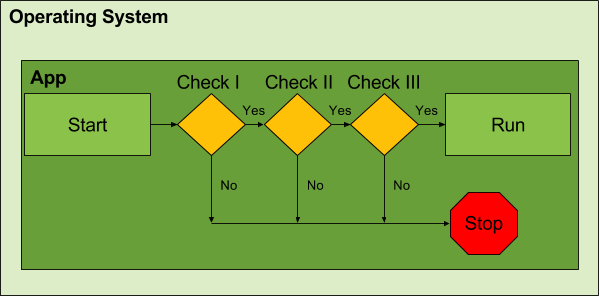
\includegraphics[width=0.8\textwidth]{data/verificationNowAdditional.png}
    \caption{Introduction of additional tests to check environment and integrity of the application}
    \label{fig:verificationNowAdditional}
\end{figure}
Since all tampering countermeasures have the \textit{yes/no} schema, they can be circumvented easily.
The goal of these checks is to increase the workload of an attacker.
The code has to be analysed in order to find, understand and patch them.
The checks can be spread inside the application to unexpectedly crash the application.
The attacker not only has to invest time to figure out why the application crashes randomly but also to find these checks.
Obfuscated and implementating it randomly increases the effort as well.
Even the possibility of implementing them in native code can be considered.
\newline
This does not prevent \gls{luckypatcherg} itself from working, but it offers an additional layer of security which has to be voided.
